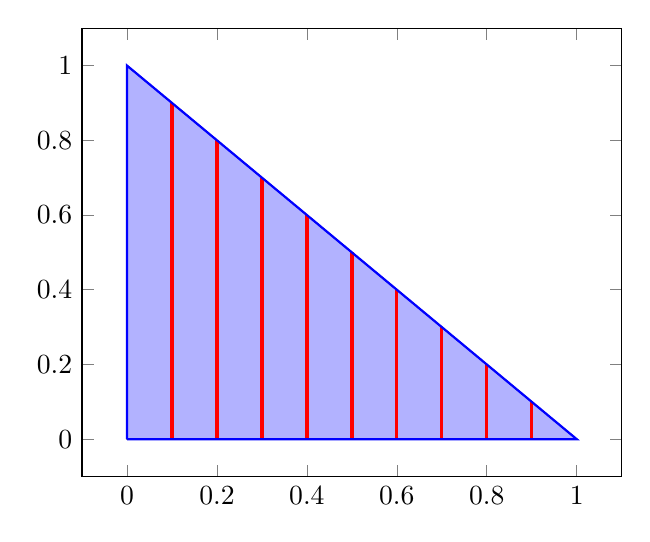
\begin{tikzpicture}
    \begin{axis}
        \draw[fill=blue!30] (axis cs:0,0) -- (axis cs:1,0) -- (axis cs:0,1) -- cycle;
        \draw[very thick,red] (axis cs: 0.1,0) -- (axis cs: 0.1,0.9);
        \draw[very thick,red] (axis cs: 0.2,0) -- (axis cs: 0.2,0.8);
        \draw[very thick,red] (axis cs: 0.3,0) -- (axis cs: 0.3,0.7);
        \draw[very thick,red] (axis cs: 0.4,0) -- (axis cs: 0.4,0.6);
        \draw[very thick,red] (axis cs: 0.5,0) -- (axis cs: 0.5,0.5);
        \draw[very thick,red] (axis cs: 0.6,0) -- (axis cs: 0.6,0.4);
        \draw[very thick,red] (axis cs: 0.7,0) -- (axis cs: 0.7,0.3);
        \draw[very thick,red] (axis cs: 0.8,0) -- (axis cs: 0.8,0.2);
        \draw[very thick,red] (axis cs: 0.9,0) -- (axis cs: 0.9,0.1);
        \addplot[blue,thick] coordinates {(0,0)(1,0)(0,1)(0,0)};
    \end{axis}
\end{tikzpicture}